\documentclass[12pt]{beamer}
\usetheme{Boadilla}
%https://www.overleaf.com/learn/latex/Beamer#Reference_guide
\usecolortheme{beaver}
%\setbeamertemplate{navigation symbols}{}
%\setbeamertemplate{headline}{}
\setbeamercovered{transparent}

\usepackage{kotex}
\usepackage{amsmath}
\usepackage{amsfonts}
\usepackage{mathtools,amssymb}

\title{Introduction}
\author{박건호}
\date{2024-2 CATDOG 리소스3D 스터디}

\begin{document}
\maketitle
\begin{frame}{Table of Contents}   
\tableofcontents
\end{frame}

\section{Blender Installation}

\begin{frame}{Blender?}
    \begin{columns}
        \column{0.5\textwidth}
            \begin{itemize}
                \item 3d tool의 많은 기능들 제공 \newline
                \item 입문하기가 제일 쉬움 \newline
                \item script를 통해 python을 이용한 프로젝트와의 연결성이 높음
            \end{itemize}

        \column{0.5\textwidth}
            \begin{figure}[t]
            \centering
            
\includegraphics[width=0.7\textwidth]{image/blender_icon.png}
            \end{figure}
    \end{columns}
\end{frame}

\begin{frame}{Install Blender}
    \begin{columns}
        \column{0.5\textwidth}
            \begin{itemize}
                \item \small{\url{https://www.blender.org/}} \newline
                \item 들어가서 Download 
            \end{itemize}

        \column{0.5\textwidth}
            \begin{figure}[t]
            \centering
            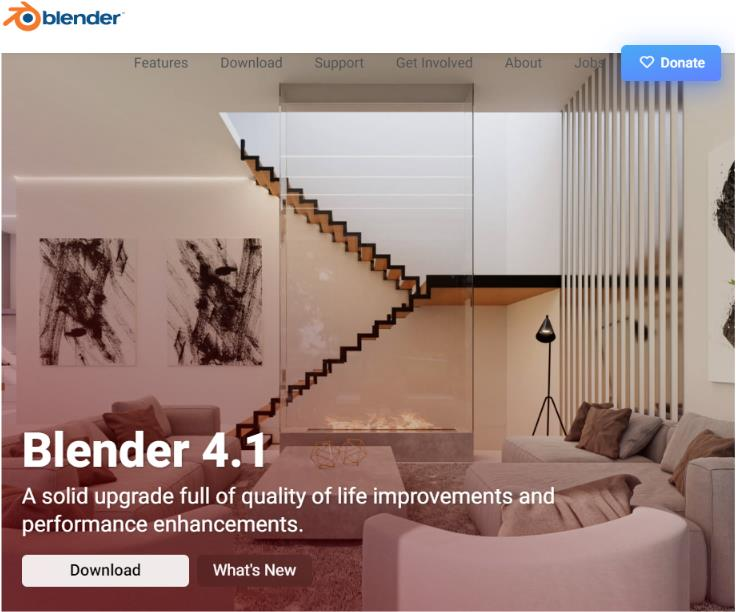
\includegraphics[width=0.7\textwidth]{image/install1.jpg}
            \end{figure}

            \begin{figure}[t]
                \centering
                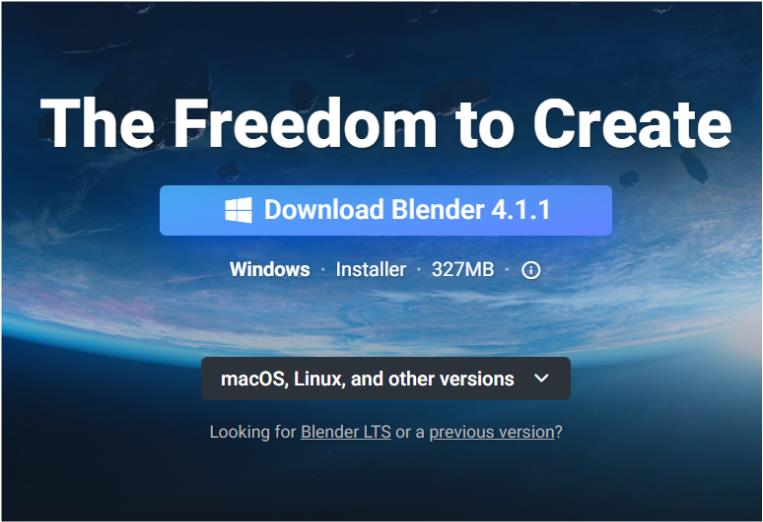
\includegraphics[width=0.7\textwidth]{image/install2.jpg}
            \end{figure}
    \end{columns}
\end{frame}

\begin{frame}{Complete!}
    \begin{figure}[t]
        \centering
        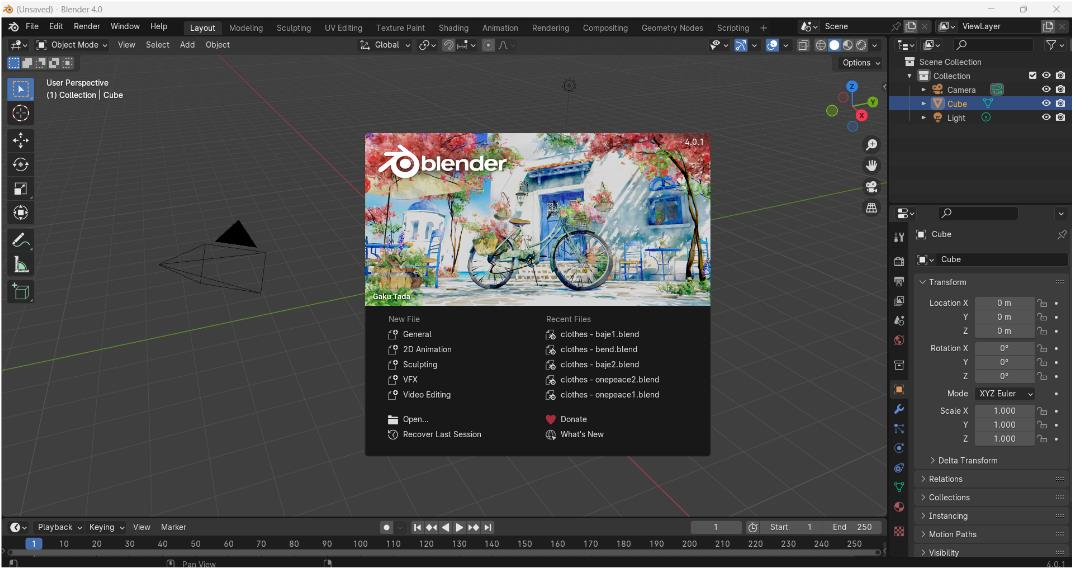
\includegraphics[width=1.0\textwidth]{image/install3.jpg}
    \end{figure}
\end{frame}

\section{github manual}

\begin{frame}{github register}
    \begin{columns}
        \column{0.5\textwidth}
            \begin{itemize}
                \item \small{\url{https://github.com/}} \newline
                \item 본인의 github 생성
            \end{itemize}

        \column{0.5\textwidth}
            \begin{figure}[t]
            \centering
            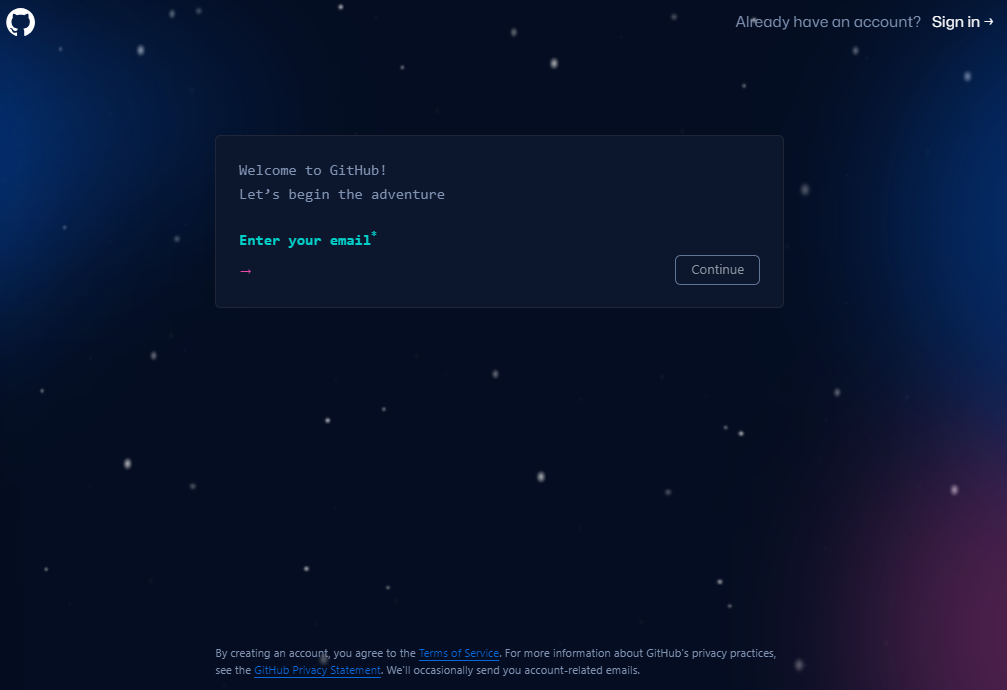
\includegraphics[width=1.0\textwidth]{image/github_register.png}
            \end{figure}
    \end{columns}
\end{frame}

\begin{frame}{create repository}
    \begin{columns}
        \column{0.5\textwidth}
            \begin{itemize}
                \item repository 생성 \newline
                \item 프로젝트 단위로 생성하는 보관함 \newline
                \item 접근 제한은 public으로 할 것 
            \end{itemize}

        \column{0.5\textwidth}
            \begin{figure}[t]
            \centering
            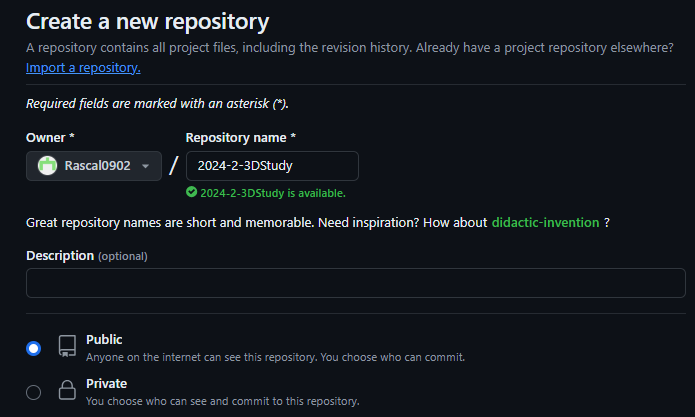
\includegraphics[width=1.0\textwidth]{image/create_repository.png}
            \end{figure}
    \end{columns}
\end{frame}

\end{document}